\lecture{13}{2025-03-31}{this year mid term will be more difficult}{}
    \section{Sequential Logic}
    \begin{parag}{Example Application: Alarm System Control}
        Suppose that we wish to control an alaram system:
        \begin{center}
            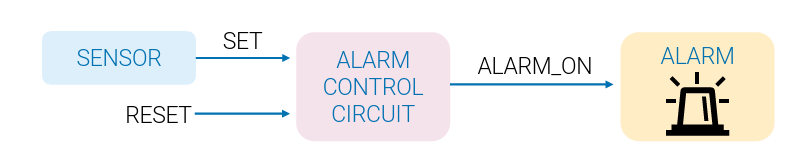
\includegraphics[scale=0.5]{12025-03-31.png}
        \end{center}
        If $ALARM\_ON = 1$, the alarm is activated; $ALARM\_ON = 0$, the alarm is deactivated.\\
        When the sense generate a positive voltage signal ($SET = 1$) in respone to some undesirable event, $ALARM\_ON$ becomes 1. \textbf{Once the alarm is triggered, it must remain active even if the sensor output returns to zero}. The alram is turned off by mans of a $RESET$ input. The circuit requires \important{a memory element} to remember that the alarm has to be active until the $RESET$ signal arrives.\\
        At this point in the course, we wouldn't be able to do so because we don't really have the sense of ``time''in combinational logic it is like a one-way function which is ``just used once''.
    \end{parag}
    \begin{parag}{Combinational vs. Sequential}
        Previously, we considered circuits where the value of each output depends solely and almost instantaneously on the values of signals applied to the inputs
        \begin{itemize}
            \item Refeerred to as \important{combinational circuits}
        \end{itemize}
        There exists another class of logic circuit in which the values of the outputs depend \textbf{not only on the} \important{present} valeus of the inputs \textbf{but  also on the} \important{past} behavior of the circuit.
    
        \begin{subparag}{Combinational circuits are \important{memoryless}}
            The outputs depends only on the present input.
        \end{subparag}
        \begin{subparag}{Sequential circuit}
            Outputs depend on the \textbf{present} and the \textbf{previous} inputs.
        \end{subparag}
        \begin{center}
            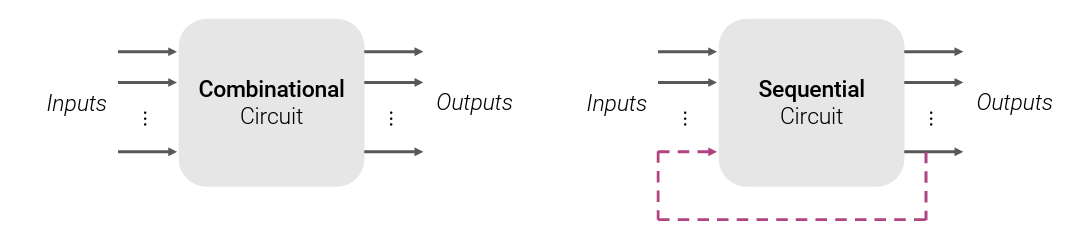
\includegraphics[scale=0.5]{22025-03-31.png}
        \end{center}
        
    \end{parag}
    \begin{parag}{Basic Memory Element}
            Here what we are looking for is a ``storage'' for the values of logic signal, it is this storage, or those stored values that \important{are the state of the circuit}. Therefore when the inputs change, the new input values either leave the circuit in the \important{same state} or cause it to change to a \important{new state}.\\
            Over time, the circuit changes through a \textbf{sequence of states} as a result of changes in the inputs.\\
        For instance, we can create a loop which inverts the input and re-inverts it etc... \\
        inverters with outputs connected to inputs:
        \begin{center}
            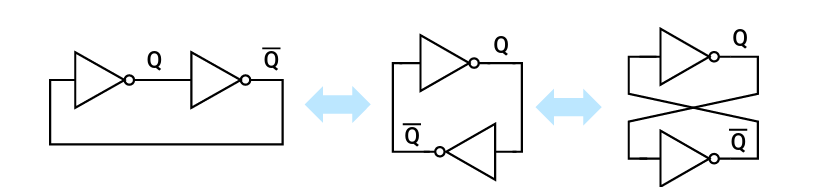
\includegraphics[scale=0.5]{32025-03-31.png}
        \end{center}
        
       However, this is not very practical because it stores a "given" value indefinitely, we cannot really access the value nor changes it so this is not really useful. What we want is to be able to access the element, therefore we need memory elements.
    
    \end{parag}
    \subsection{Memory Elements}
    \subsubsection{Latches}
    \begin{parag}{Set-Reset Latch with Reset priority}
        There is a memory element with NOR gates, \\
        Both NORs act as inverters in a bistable memory element:
        \begin{center}
            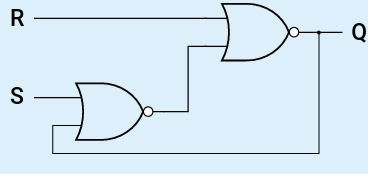
\includegraphics[scale=0.5]{42025-03-31.png}
        \end{center}
        \begin{definition}
            A table describing a sequential circuit behavior is called a \important{characteristic table}.
        \end{definition}
        How the next state changes in the function of the inputs \textbf{and} the previous state.
        \begin{center} \begin{tabular}{cc|c}$S$ & $R$ & $Q_{next}$ \\ \hline  0 & 0 &  \\ 0 & 1 &  \\ 1 & 0 & $f\left(S, R, Q\right)$ \\ 1 & 1 &  \end{tabular} \end{center} 
       \begin{subparag}{Latch}
           \begin{definition}
               Depending on the value of the output $Q$,  a latch be in one of the two states (S):
               \begin{itemize}
                   \item $S0: \; Q = 0$
                   \item $S1:\; = 1$
               \end{itemize}
               A state is a property of a memory element, State is defined by the logic value kept by the memory element $(Q)$.
           \end{definition}
       \end{subparag} 
       If we called the two NOR, $Q_b, Q_a$:
       \begin{align*}
           Q_b = \overline{S + Q_a}
       \end{align*}
       For the next $Q_a$ we get:
       \begin{align*}
           Q_{a, \; next} &= \overline{R + Q_b}\\
           &= \overline{R + \overline{S + Q_a}}\\
           &= \overline{R} \cdot (S + Q_a)\\
           &= \overline{R} \cdot S + \overline{R} \cdot Q_a = Q_{next}
       \end{align*}
       If we assume that  initially $Q_a = 0, Q_b = 1$ and \important{R is inactive (0)}.:
       \begin{itemize}
           \item When $S$ becomes $1$:
               \begin{itemize}
                   \item $Q_b$ becomes $0$, and $Q_a$ becomes $1$
               \end{itemize}
           \item While $S$ is $0$
               \begin{itemize}
                   \item $Q_a$ and $Q_b$ are complements of one another
                   \item Circuit state does not change (it is stable).
               \end{itemize}
       \end{itemize}
       
       However:
       \begin{itemize}
           \item Assume initially $Q_a = 0$, $Q_b = 1$
           \item $S$ is inactive
               \begin{itemize}
                   \item When $R$ becomes $1$:
                       \begin{itemize}
                           \item $Q_a$ becomes $0$, and $Q_b$ becomes $1$
                       \end{itemize}
                   \item While $R$ is $0$:
                       \begin{itemize}
                           \item $Q_a$ and $Q_b$ are complements of one another
                           \item Circuit state is stable
                       \end{itemize}
               \end{itemize}
       \end{itemize}
       Finally:
       \begin{itemize}
           \item Assume initially $Q_a = 0, Q_b = 1$,
           \item if both $S$ and $R$ are active:
               \begin{itemize}
                   \item $Q_a$ and $Q_b$ becomes $0$, both
               \end{itemize}
       \end{itemize}
       
       If we take the truth table:
       \begin{center}
       \begin{tabular}{cc|cc|cc}
           $S$ & $R$ & $ \overline{R} \cdot S$ & $ \overline{R} \cdot Q_a$ & $Q_{next}$ & $Q_{b, next}$ \\
           0 & 0 & 0 & $Q_a$ & $Q_a$ & $\overline{Q}_a$ \\
           1 & 0 & 1 & $Q_a$ & 1 & 0 \\
           1 & 1 & 0 & 0 & 0 & 0
       \end{tabular}
       \end{center}
       
       As you can see here, even when $S$ and $R$ are active, we still reset the output, this was a Latch we reset priority
        
    
    \end{parag}
    

    
    \begin{parag}{Set-reset latch with \important{Set} priotity}
      However it isn't always the best options to always have a reset priority, therefore we introduce also a Latch with a \important{Set} priority.
      \begin{center}
          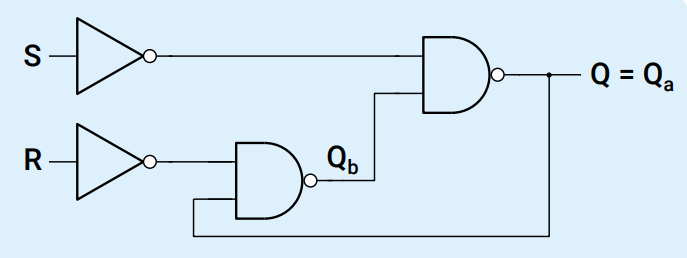
\includegraphics[scale=0.6]{12025-06-20.png}
      \end{center}
      \begin{align*} Q_{a, next} =  S + \overline{R}\cdot Q_a \end{align*}
      \begin{center} \begin{tabular}{cc|c|cc}$S$ & $R$ & $\overline{R}\cdot Q_a$ & $Q_{a, next}$ & $Q_{b, next}$ \\ 0 & 0 & $Q_a$ & $Q_a$ & $\overline{Q}_a$ \\ 0 & 1 & 0 & 0 & 1 \\ 1 & 0 & $Q_a$ & 1 & 0 \\ 1 & 1 & 0 & 1 & 1 \end{tabular} \end{center} 

      \begin{subparag}{Note}
         We usually try to avoid activating both $R$ and $S$.
      \end{subparag}
        
    \end{parag}
    
    \begin{parag}{Latches with a control signal}
        In practice, we want to  be able to control \important{when} state changes occur. To that purpose, we add a \textbf{control} signal.
        \begin{itemize}
            \item When active, it enables the latch to operate normally
            \item When inactive, it prevents states updates
        \end{itemize}
        
    \end{parag}
    \begin{parag}{$D$ latch}
        A D latch is a \important{Level sensitive} element, this means the change are allowed only when the control signal $C$ is active (at a high level).\\
        When the control signal is not active, the output $Q$ stays \textbf{unchanged}.\\
        \begin{subparag}{Personal note}
            A level sensitive element is a type of circuit components that whose behavior depends on the level of a control signal and not when it changes.\\
            For instance if you take a door, a sensitive level components would be:
            \begin{center}
                the door only opens when you press and \important{hold} a button
            \end{center}
            The button is the signal control here and opens the door \textbf{as long as the control signal is at a certain level}
           
            
        \end{subparag}
         \begin{center}
                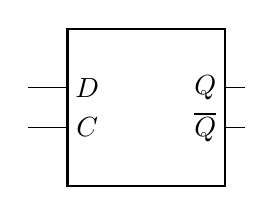
\begin{tikzpicture}
                    \draw[color=black, thick](0, 0) rectangle (2, 2);
                    \draw[](-0.5, 1.25) -- (0, 1.25) node at (0.25, 1.25) {$D$};
                    \draw[](2, 1.25) -- (2.25, 1.25) node at (1.75, 1.25) {$Q$};
                    \draw[](-0.5, 0.75) -- (0, 0.75) node at (0.25, 0.75){$C$};
                    \draw[](2, 0.75) -- (2.25, 0.75) node at (1.75, 0.75){$\overline{Q}$};
                \end{tikzpicture}
            \end{center}
            And the waveform is given as:
            \begin{center}
                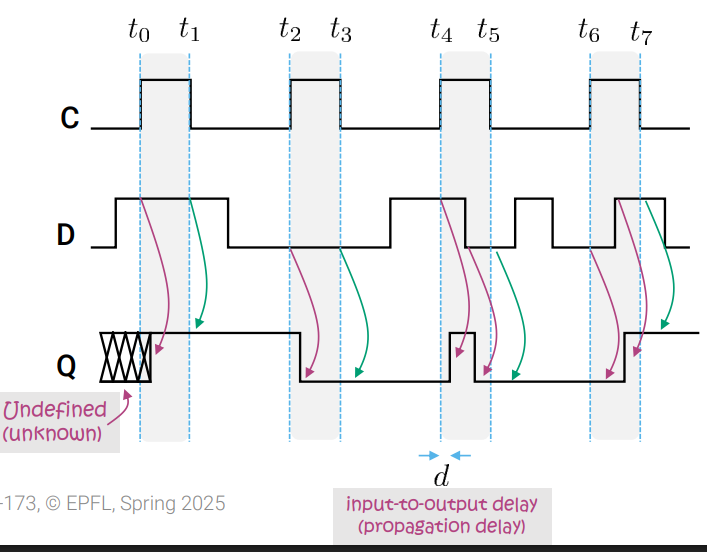
\includegraphics[scale=0.5]{22025-06-20.png}
            \end{center}
            
            
            
            
    \end{parag}
    
    \subsubsection{Flip-Flops}
    However, this issue with D latch is that as is it level sensitive, it changes more than one time while the control signal is active, in practice, limiting the duration of time when the state changes can occur is very desirable.\\
    Also, we want to memorize (keep) a state for a while and not allow it to change an unlimited number of times while the control signal is active (we will see why when we will do sequential logic)\\
    The goal it to allow the circuit to change state  only when the control signal \textbf{transition} (rising or falling edge)
    \begin{parag}{D Flip-Flop}
        A $D$ flip-flop is an \important{edge sensitive} memory element\\
        It responds to the changes at the input $D$ only when the controlling signal $C$ transitions
        
          \begin{center}
                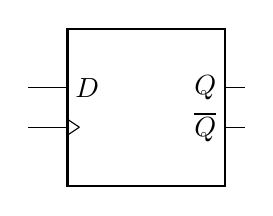
\begin{tikzpicture}
                    \draw[color=black, thick](0, 0) rectangle (2, 2);
                    \draw[](-0.5, 1.25) -- (0, 1.25) node at (0.25, 1.25) {$D$};
                    \draw[](2, 1.25) -- (2.25, 1.25) node at (1.75, 1.25) {$Q$};
                    \draw[](-0.5, 0.75) -- (0, 0.75) ;
                    \draw[](0, 0.85) -- (0.15, 0.75);
                    \draw[] (0, 0.65) -- (0.15, 0.75);
                    \draw[](2, 0.75) -- (2.25, 0.75) node at (1.75, 0.75){$\overline{Q}$};
                \end{tikzpicture}
            \end{center}
        
        \end{subparag}
        
        \begin{center}
            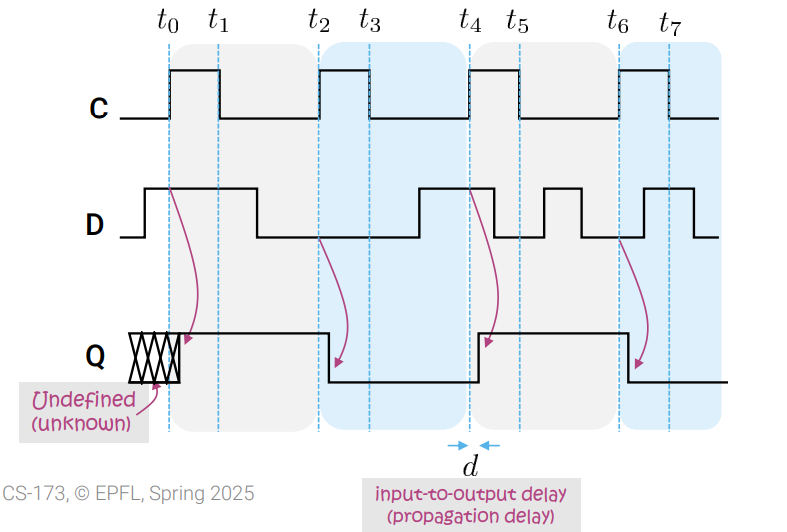
\includegraphics[scale=0.7]{32025-06-20.png}
        \end{center}
        
    \end{parag}
    
    
    

   \subsubsection{Clock}
   \begin{parag}{Clock signal}
       A Signal determine when the state changes occur is called \textbf{clock}.\\
       A clock is a periodic signal defined by its frequency (or period) and duty ratio \begin{framedremark}
       All digital system use clocks to synchronize state changes
       \begin{itemize}
           \item Typically, state changes are triggered by a rising edge of the clock.
       \end{itemize}
       
       \end{framedremark}

       
   \end{parag}
   \begin{parag}{Synchronous vs Asynchronous signal}
       \begin{itemize}
           \item A \important{synchronous signal} is one that is evaluated and updated only on the active edge (rising or falling) of the clock
           \item A \important{asynchronous signal} is one that immediately affects the output (the sate) regardless of the clock edge
       \end{itemize}
       
       
   \end{parag}
   
   
    
    
    
